\chapter{基于点云的三维深度学习}
\label{cha:3d_deep_learning}

点云本身并不是一个新概念。事实上,早期的三维激光扫描仪的原始输出正是点云。
但是,这样的仪器在当时并不普及,相关的需求也不大,因此鲜有学者对其展开深入的研究。%其服务对象通常是专业人员,而非普通大众。
而近年来,三维扫描设备得到了很大发展,甚至已经集成并嵌入到了 Kinect 和 iPhone X 等大众化产品内部,使得点云数据真正走入到人们的日常生活当中,点云三维深度学习相关的需求也呼之欲出。


\section{点云三维深度学习优劣与特点 \label{section:pcintro}}
点云具有许多优良的特性
,%使得其表现往往优于其他形式。这也
使得它成为当今三维深度学习的研究热点。

正如第 \ref{cha:intro} 章中所介绍的,点云的本质是在三维模型的二维表面上进行采样的结果。其形式上记录着三维的信息,但实则只有二维的数据量,因此是一种非常稀疏的表示。与体素和多视角图像图像相比,点云占用的空间更小,对计算资源的需求也更低。

此外,点云数据非常容易进行预处理。在二维深度学习中,数据增强是我们常使用的一个预处理技巧\cite{alexnet},例如在图像上随机切割,旋转,翻转等。这样的操作通常需要在流水线前端配置一个较为复杂的预处理程序。
但对于点云来说,简单的矩阵乘法即可完成同样的功能\cite{pointnet},而且非常容易通过现有的深度学习框架实现,并在 GPU 上高速执行。


“尺之木必有节目,寸之玉必有瑕瓋”,点云也不是十全十美的表示形式。
卷积神经网络 (Convolutional Neural Network, CNN) 的巨大成功\cite{lenet5, alexnet, vgg, googlenet, resnet},与其对局部细节的重视密不可分。在经典的卷积神经网络中,每一层中间表示的取值只于上一层附近的区域有关。由于数据是规则的,因此可以按照位置被迅速索引,高效地提取局部细节信息。%不必费除灰之力。
然而,点云数据却是无序的,因此局部细节的提取非常麻烦。在没有对各点位置进行有效索引的情况下,我们不得不遍历整个点集,效率低下。而即使借助 $k$-d 树 等数据结构实现了高效的处理,其复杂程度也远远超过了传统的情况,不便于使用 GPU 等并行计算设备进一步加速。


但是,我们应当承认,点云三维深度学习提出影响深远,意义重大。
它将不规则的几何表示与深度学习算法相结合,打破了原来深度学习只能处理规则型数据的思维定势,为我们的研究开辟了一条崭新的道路。

诚然,相对于点云而言,三角面片和基于 CAD 原语的参数化表示是三维模型更自然、更准确、更完善的表现形式。但正因为如此,它们也更复杂,更不容易被现有深度学习算法所处理。
因此,%笔者
我们认为点云是三维深度学习发展过程中一个必然的
%历史过渡
历史阶段
,是一个连接传统二维深度学习与更高级的三维深度学习之间的重要桥梁。


\section{基于图片的三维点云重建 \label{section:pointsetgen}}
本节介绍 PointSetGen\cite{pointsetgen} 工作的主要内容。
\subsection{问题描述}
PointSetGen
解决了点云的三维重建问题,是本文的主要参考对象。在这个工作中,用户需要提供一张三维物体的 RGBA 图像,即 RGB 图像与 mask 信息。 随后,算法会根据输入图像,以点云的形式重建出三维模型的完整结构,包括遮挡与不可见的部分。另外,为了简化问题,我们进一步假设生成结果中点云的点数 $N$ 为固定常数,如 $N =  \numprint{1024}$。

图 \ref{fig:pointsetgen} 是使用本算法进行重建例子。可以看到,由于遮挡等原因,输入图像中汽车的尾部并不可见,
然而这并不影响重建算法的运行。在重建结果中,汽车尾部的形状仍然清晰可见。

\subsection{模型架构}
遮挡、投影等客观因素,造成了信息的丢失,使得问题的解具有一定的多样性和不确定性。因此,此工作首先引入了一个随机变量 $\bm r \sim \NormDist(\bm 0, \bm I)$ 来刻画这样的不确定性。令输入的 RGBA 图像为 $\bm I$,输出的点云为 $S = \{(\bm p_i)\}_{i=0}^{N - 1}$,则此工作的基本流程与结构可用下式表示:
\begin{align}
	S = G(\bm I, \bm r; \bm  \theta)
\end{align}
其中 $G$ 是网络架构,$ \bm \theta$ 是需要学习出的网络参数。

基本版 PointSetGen 的网络架构 $G_{\text{vanilla}}$ 如图 \ref{fig:vanillapointsetgen} 所示。它首先通过二维深度学习中经典的卷积神经网络,将输入图像 $\bm I$ 映射为一个隐向量。随后,将计算出的隐向量通过一套全连接网络,便可以回归出最终的输出点云。尽管这个网络很简单,它的效果却出乎意料的好。
\begin{figure}[h]
	\centering%
	\subcaptionbox{基本版 PointSetGen 的网络架构 $G_{\text{vanilla}}$\label{fig:vanillapointsetgen}}
	{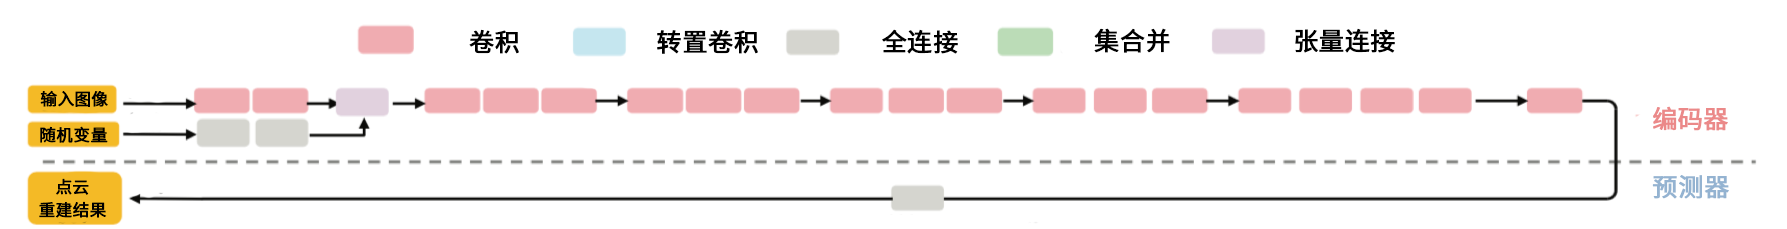
\includegraphics[width=.95\textwidth]{vanillapointsetgen}}
	\\

	\subcaptionbox{双分支版 PointSetGen 的网络架构 $G_{\text{two\_branch}}$\label{fig:tbpointsetgen}}
	{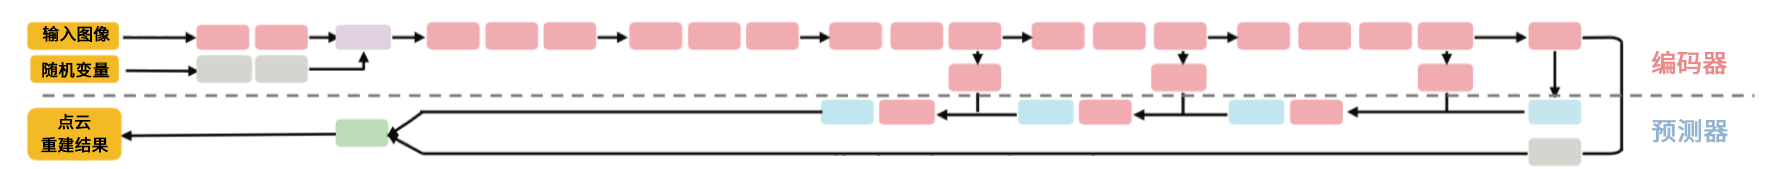
\includegraphics[width=.95\textwidth]{tbpointsetgen}}
	\\

	\subcaptionbox{Hourglass 版 PointSetGen 的网络架构 $G_{\text{hourglass}}$\label{fig:hpointsetgen}}
	{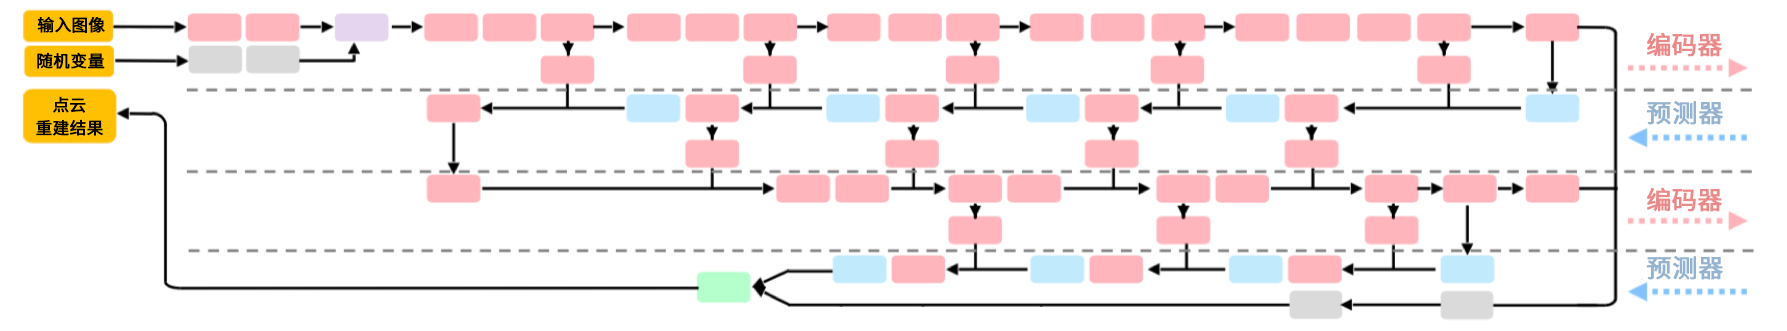
\includegraphics[width=.95\textwidth]{hpointsetgen}}
	\\

	\caption{PointSetGen\cite{pointsetgen} 的网络架构 $G$}
\end{figure}


在基本版的网络架构 $G_{\text{vanilla}}$ 中,各个点的输出是互相独立地被预测出来的,并没有任何相关性。然而在真实世界中,各点之间往往是有相关性的,如构成一个平滑表面、棱、角等。为了更好的刻画这样的相关性,双分支版本 $G_{\text{two\_branch}}$ 对全连接网络进行了调整,用一个转置卷积网络 和 更小的全连接网络进行了替换,其中前者提供 $3/4$ 的点,后者提供 $1/4$ 的点。两者组合起来便形成了最终的输出,如图 \ref{fig:tbpointsetgen} 所示。与基本版相比,双分支版的效果略有提升。



Hourglass 版本的网络架构 $G_{\text{hourglass}}$ 在已有基础上进一步提升。通过多层卷积和转置卷积操作,局部和全局的特征得到了充分的挖掘,如图 \ref{fig:hpointsetgen} 所示。其表现结果比基本版和双分支版都略有提升。


\subsection{制定衡量模型优劣的标准}
要衡量模型的优劣,并依照这个标准训练出好的模型,一个合理的损失函数是必不可少的。
% 本文
此工作
的最大贡献就是提出了两个损失函数的候选方案——Chamfer 距离 (Chamfer Distance, CD) 和 推土机距离 (Earth Mover's Distance, EMD),我们在第 \ref{cha:intro} 章中已经有所介绍:
\begin{align}
	\DCD{S_1}{S_2}  & =
	\sum_{\bm p \in S_1} 􏰘\min_{\bm q \in S_2} \Norm*{\bm p - \bm q}^2 +
	\sum_{\bm q \in S_2} 􏰘\min_{\bm p \in S_1} \Norm*{\bm p - \bm q}^2 \tag*{\ref{eq:cd}} \\
	\DEMD{S_1}{S_2} & =
	\min_{\text{双射} \phi:\, S_1 \to S_2} \sum_{\bm p \in S_1} \Norm*{\bm p - \phi(\bm p)}_2
	\tag*{\ref{eq:emd}}
\end{align}

% 设真实的结果应为 $S_{\text{gt}}$,则通过最小化 $\DCD{ S_{\text{gt}} }{S}$ 或 $\DEMD{ S_{\text{gt}} }{S}$,我们就可以得到一个合理的模型 $G(\cdot, r; \theta)$,从而解决问题。

虽然 Chamfer 距离 \eqref{eq:cd} 的求解是平凡的,但推土机距离 \eqref{eq:emd} 的值并不容易高效求得。简单分析可知,计算 \eqref{eq:emd} 等价于求解一个二分图最小权匹配的问题。能直接使用的经典算法如 %Edmonds–Karp
Kuhn-Munkres 等,至少需要 $\mathcal{O}{(N^3)}$ 的计算时间,而且很难并行化,不能发挥 GPU 的强大威力。鉴于此,这个工作进一步引入了一个近似算法实现 \eqref{eq:emd}的估算,并给出了基于 CUDA 语言的实现。限于篇幅,此处不再展开介绍近似算法的流程。

\subsection{训练模型}
由于引入了随机噪声 $\bm r \sim \NormDist(\bm 0, \bm I)$,直接使用传统的深度学习算法训练是不可取的,因为这样不能保证 $\bm r$ 能刻画出遮挡、投影等客观因素带来的多样性和不确定性。

对此,这个工作中提出了最小 $n$ 损失函数 (Min-of-N loss, MoN loss) 和 VAE 两种训练方式。使用最小 $n$ 损失训练即最小化下式:
\begin{align}
	\Loss(\bm \theta) = \sum_k
	\min_{\substack{\bm r_j \sim \NormDist(\bm 0, \bm I) \\  1 \le j \le n}}
	\DCDEMD{    G(I_k, \bm r_j; \bm \theta)    }{   S_k^{\text{gt}}   }
\end{align}
其中 $k$ 是训练数据的编号,$S_k^{\text{gt}}$ 是第 $k$ 号模型的真实点云。
而 VAE 的训练方式我们将在第 \ref{section:vae} 节中进一步展开介绍。

\subsection{训练数据集的准备 \label{section:pointsetgenpre}}
虽然我们目前已经有了充足的二维图像\cite{imagenet}和三维模型\cite{shapenet}的数据集,但这两者并没有直接的对应关系。
%在本问题里,
而在此工作中,输入图像 $I$ 与真实点云 $S^{\text{gt}}$ 是严格对应的。
如果找不到成对的二维图像和三维模型数据,我们就不能有效地%的对模型
进行训练。

在第 \ref{cha:intro} 章中,我们简要的介绍了计算机视觉与计算机图形学的历史背景与研究重点。
有趣的是,这两个学科研究的问题恰好为互逆的关系。

在计算机图形学中,通常用户会提供模型、材质、纹理、光照、摄像机视角等参数,希望计算机能尽可能自动地绘制出此场景。而在计算机视觉中,用户往往会提供一张真实拍摄的图片,并希望计算机反推出图像中的模型、材质、纹理、光照、摄像机视角等。
因此,我们能否借助图形学的手段,来完成训练数据的收集呢?

早期的 RenderForCNN \cite{rendercnn} 工作就提出了这样一个创造性的想法——通过渲染已有的三维模型,就可以得到用于训练的二维图像数据。这个工作向我们
%展示了,
证实:即使是使用计算机渲染出的图片进行训练,测试时我们仍然可以在现实生活中拍摄的图片上取得较好的结果。本节所介绍的 PointSetGen 也使用了同样的方法,完成了数据集的准备工作。


\subsection{改进方向}
%笔者
我们
认为,作为点云三维深度学习的鼻祖,此工作有非常多的亮点值得我们学习与参考,如 Chamfer 距离和推土机距离的提出,
最小 $n$ 损失函数的建立等。但
它
作为点云三维深度学习的早期工作,%此工作也难免有一定的不足。
难免会有一定的不足之处,
例如:
\begin{itemize}
	\item 此工作需要用户提供 mask 信息:用户体验差;另外
	\item 此工作对于新数据的泛化能力不强:对于训练数据集中未曾出现的新图像,重建算法有可能失败。
\end{itemize}
这两点也正是本文工作希望进行改进的方向。


\section{点云数据的分类与分割\label{section:pointnet}}
本节介绍 PointNet\cite{pointnet}  工作的主要内容。

\subsection{问题描述}
如图 \ref{fig:pointnet} 所示,PointNet 解决了点云的分类与分割问题,是图像分类、图像分割等经典问题在点云数据上的推广。

\subsection{问题的初步分析}
% TODO: 网络结构 网络架构

点云是点的集合,满足无序性。容易想到,即使将点的顺序打乱,其分类与分割结果也不应当发生任何变化。
然而,现在比较成熟的网络架构,如全连接网络、卷积神经网络、基于长短期记忆单元 (Long Short-Term Memory, LSTM)的循环神经网络 (Recurrent Neural Network, RNN)、递归神经网络 (Recursive Neural Network, RvNN) 等均不具备这样的性质。

一种直接的想法是,我们可以对于点云进行数据增强,即将原训练数据随机打乱顺序后,送入上述深度神经网络进行训练。
然而这种方法的表现并不理想。

众所周知,$N$ 个点具有 $N!$ 种可行的排列方案。而有限的时间内,能参与到训练过程的排列数肯定远远小于 $N!$。因此,这种朴素的想法很难保证所有的 $N!$ 种排列方案所对应输出的一致性。

另一种直接的想法是,我们可以对点云数据进行排序,再送入已有深度神经网络进行训练。
如果点云是一维数据,那么排序算法确实是一种有效的方法。
但对于三维数据,排序算法的表现就力不从心了。

事实上,高维数据并没有一种鲁棒的、抗干扰的排序方式。即使是字典序,一点微小扰动就会给排序结果带来巨大的改变,而这却不会很大程度地改变点云的分类与分割结果。

上述两种朴素方法的缺点,迫使着我们去思考:能否跳出已有网络架构的限制%枷锁
,
% ,提出一种新的方案
% ,从网络架构的设计出发,
直接设计出一个全新的网络架构,从源头上确保输出与输入数据顺序无关呢?本节所介绍的 PointNet 正一个这样的工作。

\subsection{模型架构}
在数学上,满足输出不随输入变量的排列而发生变化的函数被称为对称函数,如多个数之和、之积、最大值或者最小值等。对于本节问题而言,点云的分类和分割同样是一个对称函数,但它比求和、最值等平凡的对称函数要复杂很多。既然如此,那么我们能否将一个平凡的对称函数,通过适当的操作转化为复杂的对称函数呢?

正如第 \ref{cha:intro} 章中我们所介绍的,如果存在映射 $h: \mathbb{R}^3 \to \mathbb{R}^K,
	g: \underbrace{\mathbb{R}^K \times \mathbb{R}^K \times \cdots \times \mathbb{R}^K}_{N} \to \mathbb{R}^K, \gamma: \mathbb{R}^K \to \mathbb{R}$,且 $g$ 为对称函数,则映射 %$f: S \to \mathbb{R}$
\begin{align}
	f(\{\bm p_1, \ldots, \bm p_N \}) = \gamma \circ g(h(\bm p_1), \ldots, h(\bm p_N)) \tag*{\ref{eq:symmetric}}
\end{align}
亦为对称函数。

PointNet 巧妙地利用了上述结论。注意到,只要我们取 $g = \max$ 为简单的对称函数,
$h = \MLP_h(\cdot; \bm \theta_h), \gamma = \MLP_\gamma(\cdot; \bm \theta_\gamma)$ 为多层感知机 (Multilayer Perceptron, MLP)表示的普通函数,那么我们就可能实现复杂对称函数的拟合任务。
事实上,PointNet 在 \inlinecite{pointnet} 中证明了:只要我们能让 $h, \gamma$ 逼近任何函数,那么 \eqref{eq:symmetric} 就能以任意精度逼近任意对称函数,即以下定理:
\begin{theorem}
	\kaishu
	设 $\mathcal{X} = \{S: S \subseteq [0, 1]^3 \text{且} \left|S\right| = N\}$,$f: \mathcal{X} \to \mathbb{R}$ 为任何 Hausdorff 距离 $d_H(\cdot, \cdot)$ 下的连续集合函数,亦即,$\forall \epsilon >0$,$\exists \delta > 0$,$\forall S, S^\prime \in \mathcal{X}$,若 $d_H(S, S^\prime) < \delta$ 则 $\Norm*{ f(S) - f(S^\prime]) } < \epsilon$。那么,$\forall \epsilon > 0$,$ \exists $ 连续函数 $h, \gamma$,满足 $\forall S \in \mathcal{X}$:
	\begin{align}
		\Norm*{ f(S) - \gamma \left( \max_{\bm x_i \in S} \{  h(\bm x_i)  \} \right)  } < \epsilon
	\end{align}
\end{theorem}
这个定理为 PointNet 的表达能力提供了理论保障。限于篇幅原因,我们不再对此定理展开证明。

根据 $\eqref{eq:symmetric}$,我们很容易设计出基本版 PointNet 的网络架构,如图 \ref{fig:vanillapointnet} 所示。

\begin{figure}[h]
	\centering%
	\subcaptionbox{基本版 PointNet 的网络架构\label{fig:vanillapointnet}}
	{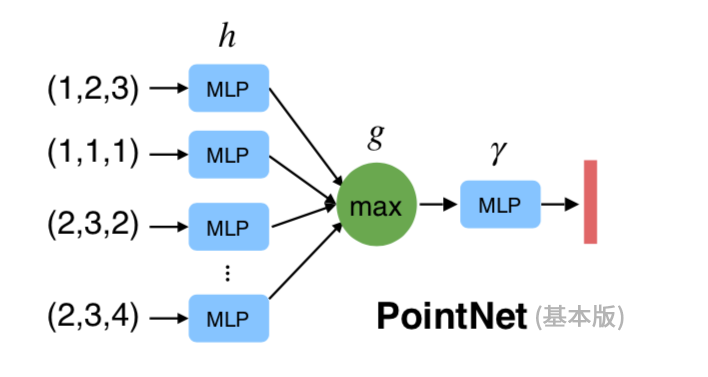
\includegraphics[width=.48\textwidth]{vanillapointnet}}%
	\hspace{0em}%
	\subcaptionbox{点云自动对齐网络\label{fig:pointnetinputalignment}}
	{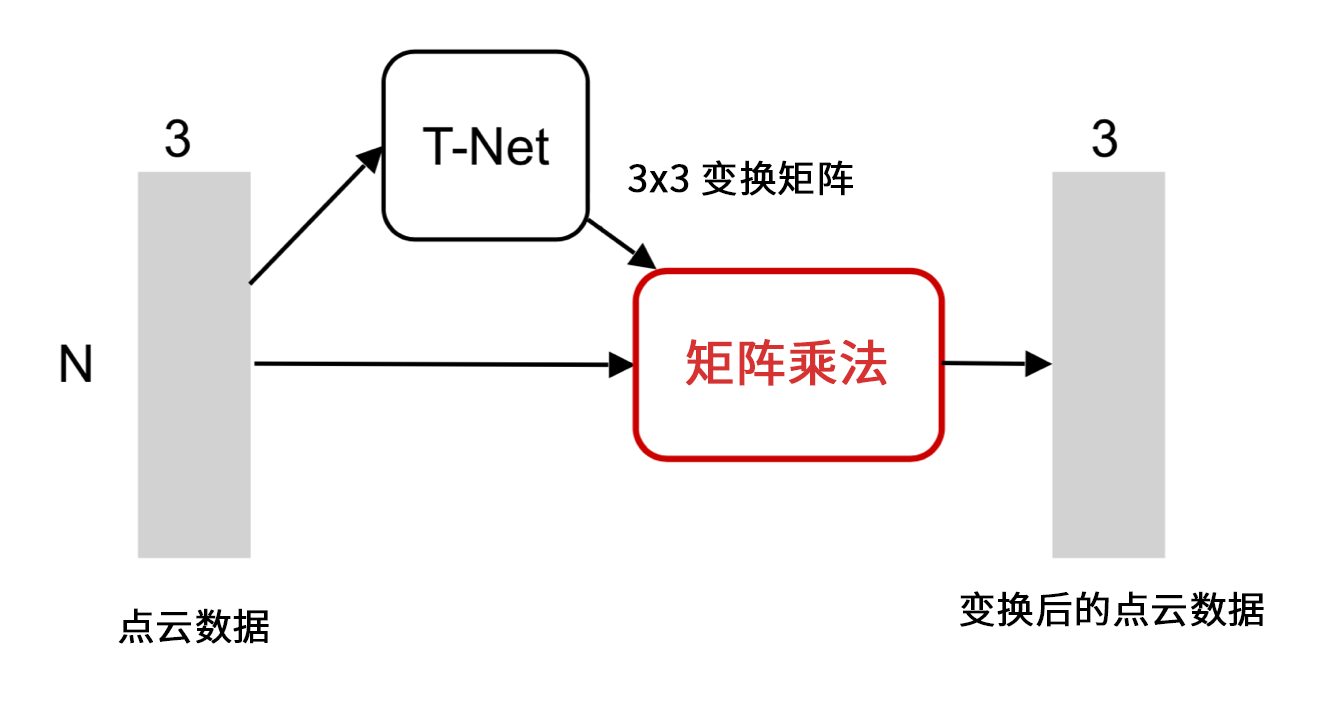
\includegraphics[width=.48\textwidth]{pointnetinputalignment}}
	\caption{PointNet\cite{pointnet} 的基本组成部件}\label{fig:pointnetelement}
\end{figure}



\subsection{点云的刚体不变性}
$\eqref{eq:symmetric}$ 只考虑了点云的排列不变性。事实上,点云数据还有刚体不变性的特点,即对任何点云数据做旋转、平移等刚体变换后,其仍然表示着同样的点云,对应的分类和分割结果不应当发生变化。

鉴于此,此工作引入了一个自动对齐点云的网络 T-Net。它可以从输入点云中自动回归出用于对齐的仿射变换矩阵。接下来只需一个矩阵乘法操作,点云的自动对齐任务就完成了,如图 \ref{fig:pointnetinputalignment} 所示。


\subsection{点云分类与分割}
通过将图 \ref{fig:pointnetelement} 中 PointNet 的基本组成部件组合,我们就得到了一个完整的点云分类与分割的网络,如图 \ref{fig:pointnetarchi}  所示。其中,对于点云分割任务来说,我们还要额外的将局部特征与全局特征相组合,确保分割结果同时兼顾到细节与整体。
\begin{figure}[h]
	\centering%
	{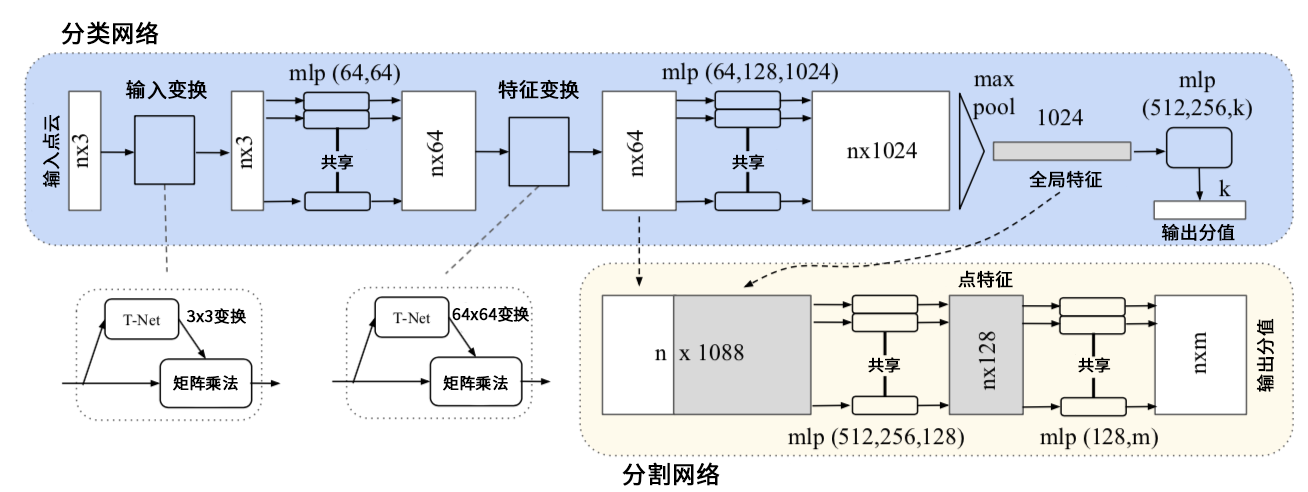
\includegraphics[width=.95\textwidth]{pointnetarchi}}
	\caption{PointNet\cite{pointnet}  的完整结构}
	\label{fig:pointnetarchi}
\end{figure}

\subsection{鲁棒性 \label{pointnet-robust}}
% \inlinecite{pointnet} 的
实验数据表明,PointNet 对点云的缺失并不敏感:即使是输入点云数据丢失了 $50\%$,其正确率也只会下降 $2\%$,如图 \ref{fig:pointnetrobust} 所示。

究其原因,我们认为是因为 $\eqref{eq:symmetric}$ 中的取最大值操作,巧妙的将模型的边、棱、角等关键点提取了出来,如图 \ref{fig:pointnetrobustvis} 第二行所示。
具体来说,对于关键点 $\bm p$ 而言,其 $h(\bm p)$ 总有一个分量值很大,因此在 $\gamma \circ \max$ 中占据了主导地位。然而,对于大部分非关键点 $\bm q$ 而言,其 $h(\bm q)$ 的各个分量值都很小,因此在 $\gamma \circ \max$ 中完全没有贡献,即它对模型的输出没有任何关联。这样的非关键点即使是缺失了,也不会对算法带来明显影响。

我们还可以进一步画出点云的上界集合,即加入后仍然不影响模型输出的点集,如图 \ref{fig:pointnetrobustvis} 第三行所示。模型对于任何介于关键点集合到上界集合的输入,都会给出同样的结果,因此 PointNet 是鲁棒的。


\begin{figure}[h]
	\centering%
	\subcaptionbox{数据丢失比例与准确率的关系\label{fig:pointnetrobust}}
	{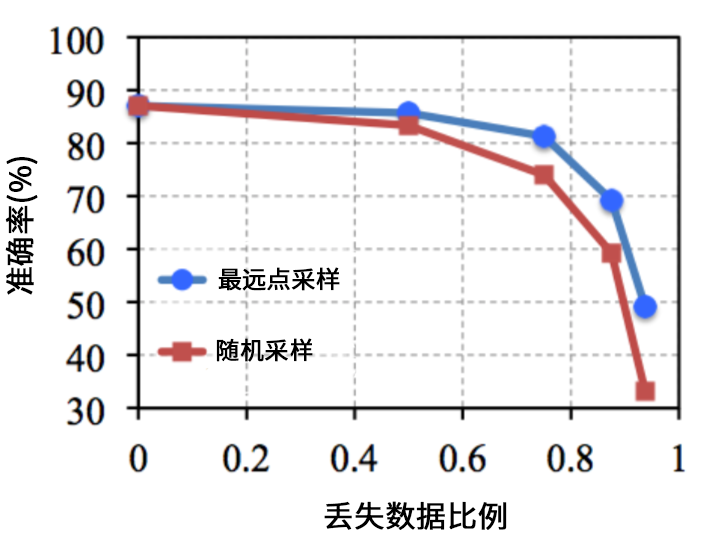
\includegraphics[width=.40\textwidth]{pointnetrobust}}%
	\hspace{2em}%
	\subcaptionbox{关键点集合与上界集合的可视化\label{fig:pointnetrobustvis}}
	{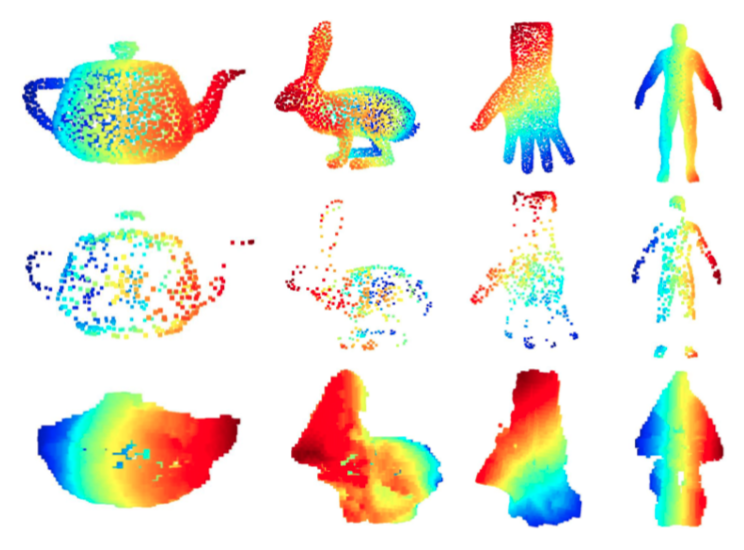
\includegraphics[width=.45\textwidth]{pointnetrobustvis}}
	\caption{PointNet\cite{pointnet}  的鲁棒性及其可视化}
\end{figure}

尽管 PointNet 鲁棒性提升了其在分类和分割问题中表现,然而在第 \ref{section:gen3d} 节中我们会看到,它 的鲁棒性会对三维点云的生成问题带来一定的麻烦。

\subsection{改进:局部细节的提取}
通过 $\eqref{eq:symmetric}$ 和图 \ref{fig:vanillapointnet},我们可以观察到:PointNet 特征提取是一种全局化方式,并不像卷积神经网络一样,重视局部细节的提取。正如我们在 \ref{section:pcintro} 节中所介绍的一样,点云的局部细节提取是很麻烦的,因此这个工作并没有对此进行过多的考虑。

事实上,目前已经有相当多的工作对于点云的局部细节提取作出了改进,如:
PointNet++\cite{pointnet2}、Kd-Net\cite{kdnet}、PointCNN\cite{pointcnn}、DGCNN\cite{dgcnn} 等。
限于篇幅,我们不再对它们逐个展开介绍。

\section{其他问题与未来展望}
除了点云生成、分类、分割以及将在第  \ref{section:gen3d} 节中详细介绍的点云生成外,目前有相当多的新工作,成功地用点云解决了更多也更具有挑战性的%点云三维深度学习
问题,
如点云场景检索\cite{pointnetvlad}、点云物体检测\cite{frustumpointnet}等。激动人心的是,现在已经有前沿工作,将点云三维深度学习中的思想和方法应用于基于三角面片的三维深度学习问题中,
如 AtlasNet\cite{atlasnet} 等。这向我们展示了点云的强大威力,同时也见证了点云对于三维深度学习发展所做出的不可磨灭的贡献。

也许有一天,点云会完成其历史使命,并悄然无息地退出三维深度学习的舞台。而取而代之的将是三角面片等更高级、更自然、更准确、更完善的三维模型表示方式。
但我们相信,没有点云相关工作的推进,就很难有三维深度学习的美好未来。

% 其他:点云检索,点云识别
